Arbeidsområdet er på grensa mellom aktiv og cutoff.
\\
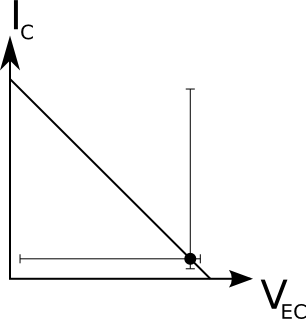
\includegraphics[width=0.5\textwidth]{./img/typeBLastlinje}
\\
I en klasse B emitterfølger blir det en effektforsterkning som kun
virker på halvperioder.
Output signalet tar ikke med negativt input signal.
\\\\
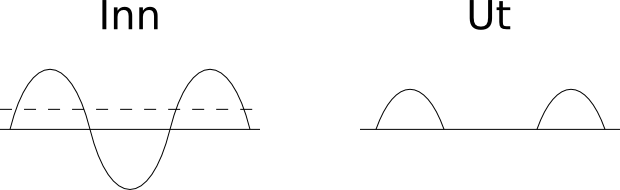
\includegraphics[width=0.67\textwidth]{./img/klasseBSignal}
\\\\
En slik forsterker ser slik ut
\\
\begin{circuitikz} \draw
(4,3) node[npn] (npn) {}
      (npn.base) node[anchor=east] {}
      (npn.collector) node[anchor=south] {}
      (npn.emitter) node[anchor=north] {}

(0,0) node[ground] {}
      to[vsourcesin, l=$V_{inn}$] (0,3)
      -- (npn.base)
(npn.collector) to[short, -o, l=$V_{CC}$] (4,4)
(npn.emitter) -- (4,2)
      to[R, l=$R_E$] (4,0)
      node[ground] {}
(4,2) to[short, -o, l=$V_{ut}$] (5,2)
      ;
\end{circuitikz}
\\\\
Det finnes også \emph{Push-Pull} klasse B forsterkere.
De bruker både npn og pnp og fanger både positive og negative signaler, men
med \emph{crossover} forvrengning.
\\\\
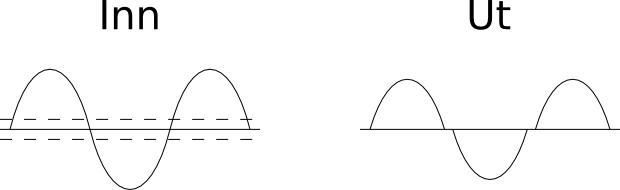
\includegraphics[width=0.67\textwidth]{./img/crossover}
